% \begin{featurebox}
% \caption{The Rules of Engagement for Order-Of-Magnitude Estimates}
% This work relies heavily on "back-of-the-envelope" estimates to understand
% the growth-rate dependent abundances of molecular complexes. This moniker
% arises from the limitation that any estimate should be able to fit on the
% back of a postage envelope. As such, we must draw a set of rules governing
% our precision and sources of key values.
%
% \textbf{\itshape The rule of "one, few, and ten".} The philosophy behind
% order-of-magnitude estimates is to provide an estimate of the appropriate scale,
% not a prediction with many significant digits \citep{mahajan2010}. We therefore define three different
% scales of precision in making estimates. The scale of "one" is reserved for
% values that range between 1 and 2. For example, If a particular process has been
% experimentally measured to transport 1.87 protons for a process to occur, we approximate
% this process to require 2 protons per event. The scale of "few" is reserved for
% values ranging between 3 and 7. For example, we will often use Avogadro's number
% to compute the number of molecules in a cell given a concentration and a volume.
% Rather than using Avogadro's number as $6.02214 \times 10^{23}$, we will
% approximate it as $5 \times 10^{23}$. Finally, the scale of "ten" is reserved
% for values which we know within an order of magnitude. If a particular protein
% complex is present at 883 copies per cell, we say that it is present in
% approximately $10^3$ copies per cell. These different scales will be used
% to arrive at simple estimates that report the expected scale of the
% observed data. Therefore, the estimates  presented here should not be viewed as
% hard-and-fast predictions of precise copy numbers, but as approximate lower (or upper)
% bounds for the number of complexes that may be needed to satisfy some cellular requirement.
%
% Furthermore, we use equality symbols ($=$) sparingly and frequently defer to
% an approximation ($\approx$) symbol when reporting an estimate, indicating that
% we are confident in the estimate to within a factor of a few.
% % or scaling ($\sim$) symbols when reporting an
% % estimate.
% % When $\approx$ is used, we are implicitly stating that
% % we are confident in this estimate within a factor of a few. When a scaling
% % symbol $\sim$ is used, we are stating that we are confident in our estimate to
% % within an order of magnitude.
%
% \textbf{\itshape The BioNumbers Database as a source for values.} In making our
% estimates, we often require approximate values for key cellular properties, such
% as the elemental composition of the cell, the average dry mass, or approximate
% rates of synthesis. We rely heavily on the BioNumbers Database
% (\href{https://bionumbers.hms.harvard.edu}{bionumbers.hms.harvard.edu},
% \cite{milo2010}) as a repository for such information. Every value we draw from this database has
% an associated BioNumbers ID number, abbreviated as BNID, and we provide this
% reference in grey-boxes in each  figure.
%
% \textbf{\itshape Uncertainty in the data sets and the accuracy of an estimate.}
% The data sets presented in this work are the products of careful experimentation
% with the aim to report, to the best of their ability, the absolute copy numbers
% of proteins in the cell. These data, collected over the span of a few years,
% come from different labs and use different internal standards, controls, and
% even techniques (discussed further in the Appendix Section "Experimental Details
% Behind Proteomic Data"). As a result, there is notable disagreement in the
% measured copy numbers for some complexes across data sets. In assessing whether
% our estimates could explain the observed scales and growth-rate dependencies, we
% also considered the degree of variation between the different data sets. For
% example, say a particular estimate undercuts the observed data by an order of
% magnitude. If all data sets agree within a factor of a few of each other, we
% revisit our estimate and consider what me may have missed. However, if the data
% sets themselves disagree by an order of magnitude, we determine that our
% estimate is appropriate given the variation in the data.
% \label{box:estimate_rules}
%
% \textbf{\itshape  Point versus continuum estimates}
% For each estimate performed in this work, we begin with a simple
% order-of-magnitude estimate for the abundance of the complex in question at
% an archetypal growth rate of around 0.5 hr$^{-1}$, followed by a more refined
% estimate across a continuum of growth rates from around 0.05 to 2.0
% hr$^{-1}$. The former estimate, always outlined in the associated figure and
% indicated as a translucent brown point in the corresponding plots, will rely
% on making coarse-grained approximations of cell mass, cell volume, and/or
% typical surface areas. The continuum estimates, displayed as a grey curve on
% the various plots, relax these assertions and incorporate empirical findings
% from the literature of how cell masses, volumes, and surface areas scale with
% the cellular growth rate. Thus, it is possible for the point estimate at a
% growth rate of 0.5 hr$^{-1}$ may not perfectly agree with the continuum
% estimate at 0.5 hr$^{-1}$. We emphasize that both the point and continuum
% estimates are not hard predictions for the complex abundance, but rather
% reflect an order-of-magnitude estimates. While the proteomic measurements
% will often not fall directly on the curve corresponding to the continuum
% estimate, we do not view this as a failure of the approach. Rather, we gauge
% the accuracy of our estimates by examining whether the 1) the point
% \textit{and} continuum estimates are within the same order of magnitude as
% the observations and 2) whether the continuum estimate qualitatively captures
% the growth-rate dependence observed in the data. We direct the reader to the
% Appendix Section "Extending Estimates to a Continuum of Growth Rates" for a more
% in-depth discussion of point versus continuum estimates.
%
% \end{featurebox}
%

\section{Nutrient Transport}
Throughout our estimates we will consider an archetypal growth rate of $\approx$
0.5 hr$^{-1}$ corresponding to a doubling time of $\approx$ 5000 seconds, as the
data sets examined here heavily sample this growth regime. We will also consider
how these values will vary at other growth rates due to changes in cell size,
surface area, and chromosome copy number \citep{taheriaraghi2015, harris2018}
(described further in the Appendix Section "Extending Estimates to a Continuum
of Growth Rates"). Here we begin by considering the critical transport processes
diagrammed in \FIG{categories}(B).

In order to build new cellular mass, the molecular and
elemental building blocks must be scavenged from the environment in different
forms. Carbon, for example, is acquired via the transport of carbohydrates
and sugar alcohols with some carbon sources receiving preferential treatment
in their consumption \citep{monod1947}. Phosphorus, sulfur, and nitrogen, on
the other hand, are harvested primarily in the forms of inorganic salts,
namely phosphate, sulfate, and ammonium/ammonia \citep{jun2018,
assentoft2016, stasi2019, antonenko1997, rosenberg1977, willsky1973}. All of
these compounds have different membrane permeabilities \citep{phillips2018}
and most require some energetic investment either via ATP hydrolysis or
through the proton electrochemical gradient to bring the material across the
hydrophobic cell membrane.

The elemental composition of \textit{E. coli} has received much quantitative
attention over the past half century \citep{neidhardt1991, taymaz-nikerel2010,
heldal1985, bauer1976}, providing us with a starting point for estimating how
many atoms of each element must be scavenged from the environment: $\approx$
50\% carbon [BioNumbers ID (BNID): 100649; obtained from the BioNumbers database,
\cite{milo2010}], $\approx$ 15\% nitrogen (BNID: 106666), $\approx$ 3\% phosphorus
(BNID: 100653), and 1\% sulfur (BNID: 100655) with the remainder being
attributable to oxygen, hydrogen, and various transition metals.  Here we
estimate the abundance and growth rate dependence of a variety of transporters
responsible for carbon uptake, and provide more extensive investigation of the
other critical elements in the Appendix
Section "Additional Estimates of Fundamental Biological Processes". Using
$\approx$ 0.3 pg as the typical \textit{E. coli} dry mass at a growth rate of
$\approx$ 0.5 hr$^{-1}$ (BNID: 103904), coupled with the approximation that
$\approx$ 50\% of this mass is carbon, we estimate that $\approx 1\times
10^{10}$ carbon atoms must be brought into the cell in order to double all of
the carbon-containing molecules.

Typical laboratory growth conditions provide carbon as a single class of sugar
(such as glucose, galactose, or xylose) often transported cross the cell
membrane by a transporter complex specific to that particular sugar. One such
mechanism of transport is via the phosphotransferase system (PTS), which is a
highly modular system capable of transporting a diverse range of sugars with
high specificity \citep{escalante2012}. The glucose-specific component of this
system transports $\approx$ 200 glucose molecules ($\approx$ 1200 carbon atoms)
per second per transporter (BNID: 114686). Making the assumption that this is a
typical sugar transport rate for the PTS system, coupled with the need to
transport $\approx 1 \times 10^{10}$ carbon atoms, we then expect on the order
of $\approx$ 2000 transporters must be expressed per cell in order to bring in
enough carbon atoms. We find, however, that the experimental measurements exceed
this by several fold [\FIG{nutrient_cellwall_energy}(A)], implying that the cell
is capable of transporting more carbon atoms than strictly needed for
biosynthesis. This holds true even at the fastest growth rates, with cells
exhibiting no apparent growth rate dependence. This constancy in the expression
appears to be specific to glucose transporters, which are known to be the
preferential carbon source \citep{monod1947, liu2005a, aidelberg2014}, and
stands in contrast with other species of transporters for glycerol, xylose, or
fructose which we find match the required transporter abundances according to
the achieved doubling time (adjusting for the specific carbon source in terms of
number of carbon atoms per molecule and the rate of transport for the particular
transporter species) [Figure Supplement S1]. This also contrasts with our
observations for uptake of phosphorus and sulfur, which turn out to align well
with our expectations across different growth conditions
[\FIG{nutrient_cellwall_energy}(B,C) and discussed further in the Appendix
Section "Additional Estimates of Fundamental Biological Processes"].

\begin{figure}
  \begin{fullwidth}
    \centering{
    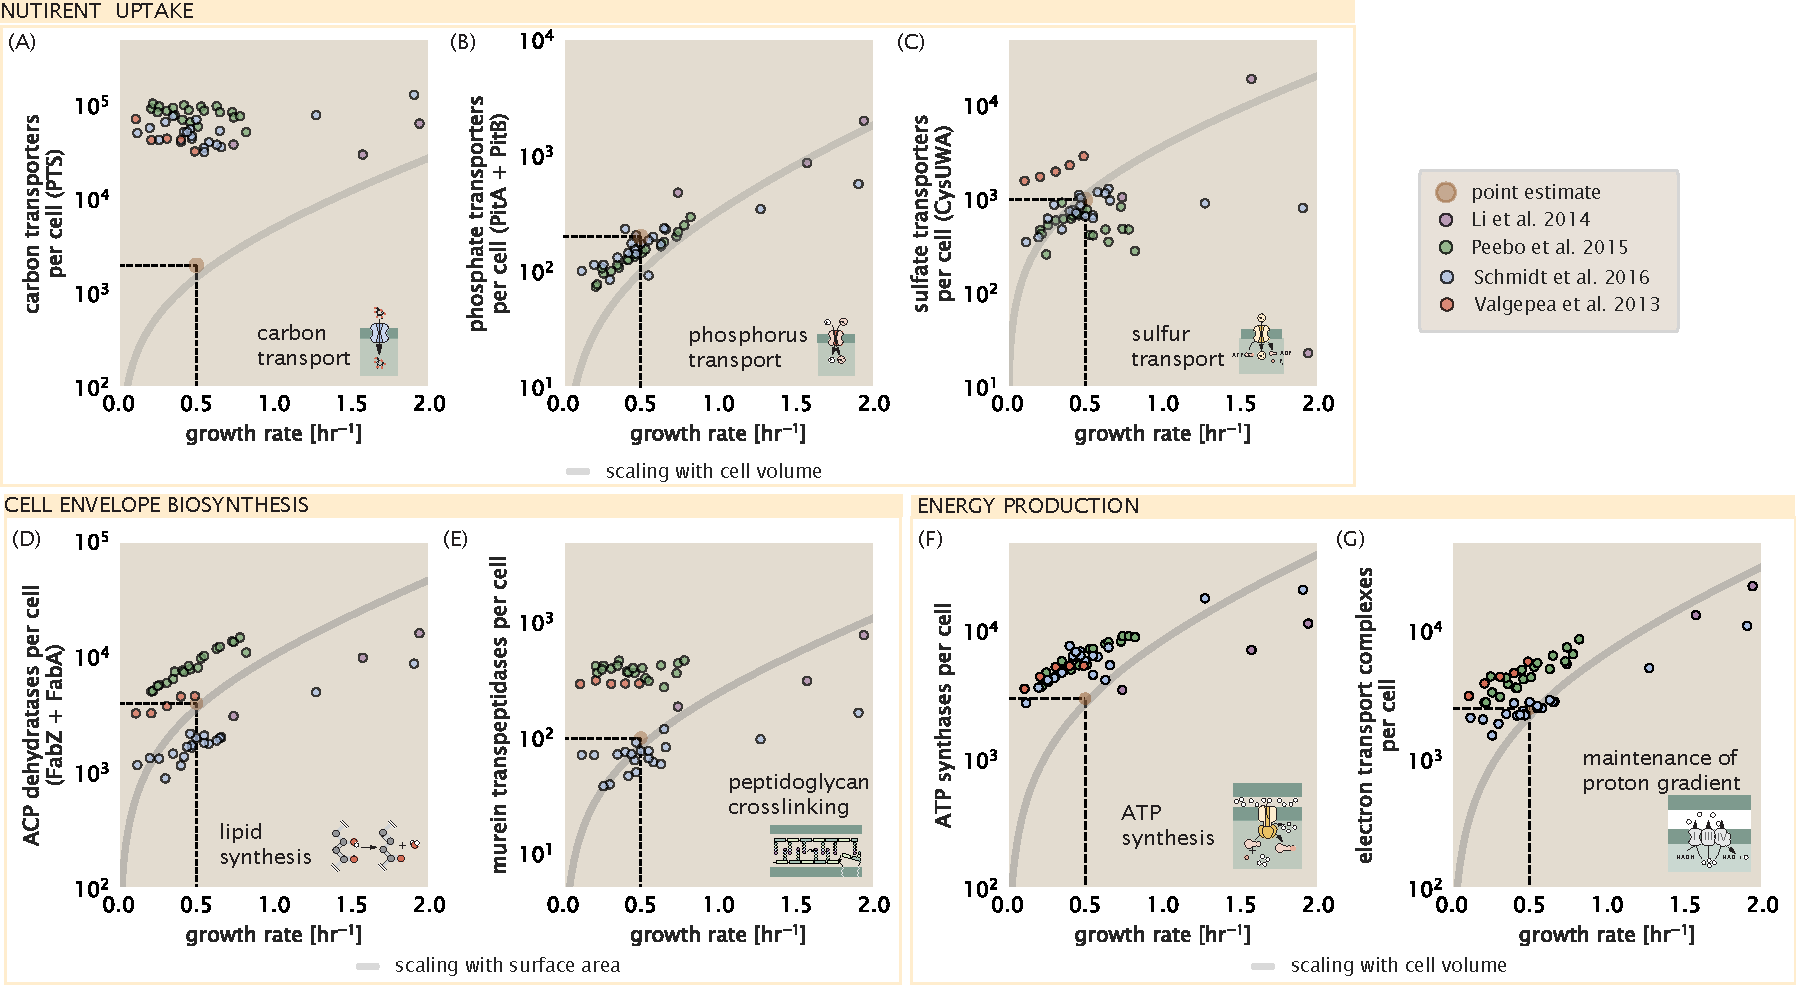
\includegraphics[width=1\textwidth]{main_figs/fig2_nutrient_cellwall_energy.pdf}
    \caption{\textbf{Key processes required for nutrient uptake, cell wall biogenesis
        and energy synthesis during growth.}
        (A) Estimate for the minimum number of generic carbohydrate
            transport systems. Colored points correspond to the mean number of complexes involved in carbohydrate
            import (complexes annotated with the Gene Ontology terms GO:0009401 and
            GO:0098704) for different growth conditions across different published
            datasets.
        (B) Number of PitA
            phosphate transport systems needed to maintain a 3\% phosphorus dry mass.
        (C) Number of CysUWA complexes
            necessary to maintain a 1\% sulfur \textit{E. coli} dry mass
            and the experimentally observed complex copy numbers using the
            transporter stoichiometry [CysA]$_2$[CysU][CysW][Sbp/CysP].
        (D) Number of ACP dehydratases necessary to form functional
            phospholipids, which is assumed to be a rate-limiting step on
            lipid synthesis, and the experimentally observed complex copy numbers using the
            stoichiometries [FabA]$_2$ and [FabZ]$_2$.
        (E) Number of peptidoglycan transpeptidases needed to complete
            maturation of the peptidoglycan and experimental measurements of the
            transpeptidase complexes, following the stoichiometries [MrcA]$_2$,
            [MrcB]$_2$, [MrdA]$_1$, and [MrdB]$_1$.
        (F) Number of F$_1$-F$_0$ ATP synthase
            complexes needed to accommodate peptide bond formation and other NTP
            dependent processes  and  experimental measurements following the
            stoichiometry
            [AtpE]$_{10}$[AtpF]$_2$[AtpB][AtpC][AtpH][AtpA]$_{3}$[AtpG][AtpD]$_3$.
        (G) Number of electron transport chain complexes
            needed to maintain a membrane potential of $-$200 mV. Points in plot correspond
            to the average number of complexes identified as being involved in aerobic
            respiration by the Gene Ontology identifier GO:0019646. These complexes include
            cytochromes \textit{bd1} ([CydA][CydB][CydX][CydH]), \textit{bdII}
            ([AppC][AppB]), \textit{bo$_3$},([CyoD][CyoA][CyoB][CyoC]) and NADH:quinone
            oxioreducase I
            ([NuoA][NuoH][NuoJ][NuoK][NuoL][NuoM][NuoN][NuoB][NuoC][NuoE][NuoF][NuoG][NuoI])
            and II ([Ndh]). Dashed lines indicate order of magnitude estimate needed at a
            growth rate of $\approx 0.5 $ per hr (light-brown point), while the gray line
            accounts for the growth rate dependence changes in cell size and doubling time.}
    \label{fig:nutrient_cellwall_energy}
    }
  \end{fullwidth}
\end{figure}

% So far we have neglected many specifics of the
% regulation of these transport systems. Using the diverse array of growth
% conditions available in the data, we also explored how individual carbon
% transport systems depend on specific carbon availability.
% A striking observation, shown in [Supp2(A)], is the constancy in the expression of
% the glucose-specific transport systems. Additionally, we note that the
% total number of glucose-specific transporters is tightly distributed at
% $\approx 1\times 10^4$ per cell, the approximate number of transporters
% needed to sustain rapid growth of several divisions per hour. Interestingly,
% this illustrates that \textit{E. coli} maintains a substantial number of
% complexes present for transporting glucose regardless of growth condition,
% which is known to be the preferential carbon source \citep{monod1947,
% liu2005a, aidelberg2014}. This stands in
% contrast with other species of transporters for glycerol, xylose, or
% fructose which we find match the required transporter abundances according to the achieved doubling time (adjusting for the specific carbon source in terms of number of carbon atoms per molecule and
% the rate of transport for the particular transporter species).

%
% Many metabolic operons, however, are regulated with dual-input logic gates that are
% only expressed when glucose concentrations are low and the concentration of
% other carbon sources are elevated \citep{gama-castro2016, zhang2014a,
% gama-castro2016, belliveau2018, ireland2020}.
% In contrast, when other carbon source (glycerol, xylose, or
% fructose) are present as the sole source of carbon, we find that cells


% Points colored in red in
% \FIG{carbon_tport}(B) (labeled by red text-boxes) correspond to growth
% conditions in which the specific carbon source (glycerol, xylose, or
% fructose) is present as the sole source of carbon. The grey lines in
% \FIG{carbon_tport}(B) show the estimated number of transporters needed at
% each growth rate to satisfy the cellular carbon requirement, adjusted for the
% specific carbon source in terms of number of carbon atoms per molecule and
% the rate of transport for the particular transporter species.
% These plots
% show that, even in the absence of the particular carbon source, expression of the
% transporters is maintained on the order of $\approx 1 \times 10^2$ per cell. The low but
% non-zero abundances may reflect the specific regulatory logic involved,
% requiring that cells are able to transport some minimal amount of an
% alternative carbon source in order to induce expression of these alternative
% carbon-source systems when needed \citep{laxhuber2020}.

% \subsection{Limits on Transporter Expression}
If acquisition of nutrients was acting as a bottleneck on cellular growth, the growth rate could be theoretically
increased simply by expressing more transporters, but is this feasible at a
physiological level? A way to approach this question is to compute the amount of
space in the bacterial membrane that could be occupied by nutrient transporters.
Considering a rule-of-thumb for the surface area of \textit{E. coli} of about 5
\textmu m$^2$ (BNID: 101792), we expect an areal density for 2000 transporters
to be approximately a few hundred transporters per \textmu m$^2$. For a typical transporter
occupying about 50 nm$^2$, this amounts to about only $\approx$ 1\% of the total
inner membrane surface area \citep{szenk2017}. In contrast, bacterial cell membranes
typically have densities of $\approx 1 \times 10^5$ proteins/\textmu m$^2$ \citep{phillips2018},
with roughly 60 \% of the surface area occupied by protein (BNID: 100078),
implying that the cell could easily accommodate more transporters. There are,
however, additional constraints on the space that  can be devoted to nutrient
uptake due to occupancy by proteins involved in processes like cell wall
synthesis and energy production, and we will consider this further in the coming
sections.
